% Drawing 80/01-2 -- folder 80, batch 01, archive page 11 (PDF page 12).
% Transcription: page de dessins au crayon, avec quelques calculs : une sphère parcourue de trois grands cercles (points d'intersection marqués) ; une pyramide et une bipyramide ; un réseau oblique de points marqués alternativement « $+$ » et « $\bullet$ » ; un octaèdre repassé à l'encre bleue, inscrit dans un cube au crayon, avec à côté un signe \uncertain{$\mathfrak{S}$} ; un cube quadrillé ; en bas à droite un polyèdre à faces carrées et hexagonales (un octaèdre tronqué ?) inscrit dans un cube ; en haut à droite un arbre ramifié à trois niveaux
% Kind: page of pencil drawings of polyhedra. Method 2 (schematic redraw from the facsimile). Status: partial.
% Notes: Whole page, schematic: a sphere with three great circles and marked intersection points (top left); a pyramid / bipyramid (below it); a three-level branching tree (top right); an oblique lattice of points marked alternately + and dot (left); the octahedron retraced in ink (heavy), with the S-like sign beside it - the pencil cube around it is not drawn; a cube with grid lines (bottom left); the polyhedron with square and hexagonal faces (bottom right) drawn as its outline and a few inner edges only. The calculations (48 = 2.4!, 5!/2.4!, 8x3x2 ...) are left out. Edges of the pencil solids are approximate.
% Coordinates: 1 unit = 1 mm = 1/100 of the crop width (bbox in page fractions: [0.05, 0.05, 0.95, 0.88]).
% Redrawn by Claude (claude-opus-5-5), issue #73, 2026-11-07; not checked by a human; not compiled (no TeX in the session).
% Rights: reproduces part of the work -- behind RENDER_TRANSCRIPTS, never published by itself.
\documentclass[tikz,border=3pt]{standalone}
\usepackage{amsmath,amssymb}
\usetikzlibrary{patterns,arrows.meta}
\tikzset{pencil/.style={black!45}, struck/.style={black!35}, mark/.style={circle,draw,inner sep=1.3pt}, pt/.style={circle,fill,inner sep=0.9pt}, opt/.style={circle,draw,fill=white,inner sep=1.1pt}}
\begin{document}
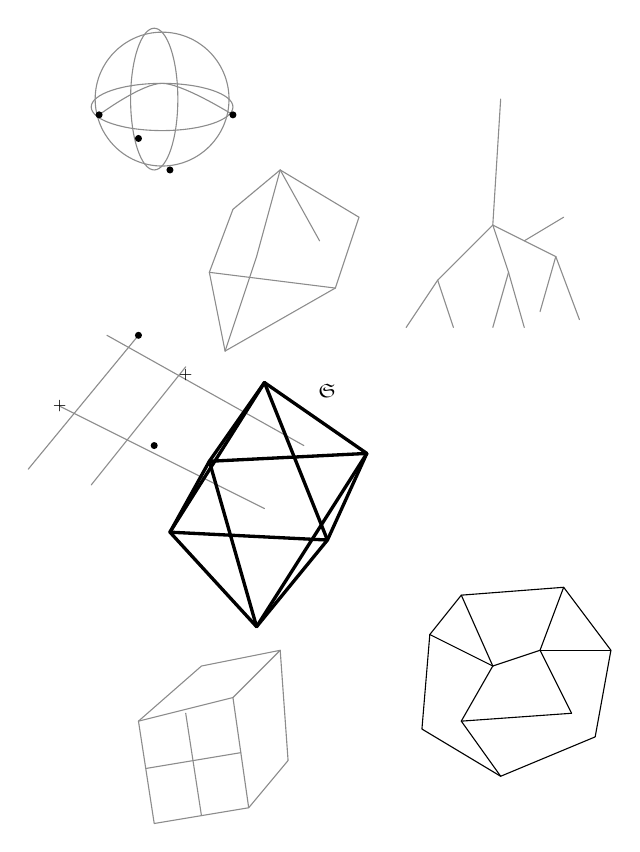
\begin{tikzpicture}[x=1mm,y=1mm,line cap=round,line join=round,font=\scriptsize]
\draw[pencil] (22,-20) circle[radius=8.5];
\draw[pencil] (21,-20) ellipse[x radius=3, y radius=9];
\draw[pencil] (22,-21) ellipse[x radius=9, y radius=3];
\draw[pencil] plot[smooth, tension=0.55] coordinates {(14,-22) (22,-18) (31,-22)};
\node[pt] at (14,-22) {};
\node[pt] at (31,-22) {};
\node[pt] at (23,-29) {};
\node[pt] at (19,-25) {};
\draw[pencil] (37,-29) -- (31,-34);
\draw[pencil] (37,-29) -- (47,-35);
\draw[pencil] (37,-29) -- (34,-40);
\draw[pencil] (37,-29) -- (42,-38);
\draw[pencil] (31,-34) -- (28,-42);
\draw[pencil] (47,-35) -- (44,-44);
\draw[pencil] (28,-42) -- (44,-44);
\draw[pencil] (28,-42) -- (30,-52);
\draw[pencil] (44,-44) -- (30,-52);
\draw[pencil] (34,-40) -- (30,-52);
\draw[pencil] (65,-20) -- (64,-36);
\draw[pencil] (64,-36) -- (57,-43);
\draw[pencil] (64,-36) -- (66,-42);
\draw[pencil] (64,-36) -- (72,-40);
\draw[pencil] (57,-43) -- (53,-49);
\draw[pencil] (57,-43) -- (59,-49);
\draw[pencil] (66,-42) -- (64,-49);
\draw[pencil] (66,-42) -- (68,-49);
\draw[pencil] (72,-40) -- (70,-47);
\draw[pencil] (72,-40) -- (75,-48);
\draw[pencil] (68,-38) -- (73,-35);
\draw[pencil] (5,-67) -- (19,-50);
\draw[pencil] (13,-69) -- (25,-54);
\draw[pencil] (9,-59) -- (35,-72);
\draw[pencil] (15,-50) -- (40,-64);
\node[inner sep=1pt] at (9,-59) {\tiny $+$};
\node[inner sep=1pt] at (25,-55) {\tiny $+$};
\node[pt] at (19,-50) {};
\node[pt] at (21,-64) {};
\draw[very thick] (35,-56) -- (23,-75);
\draw[very thick] (35,-56) -- (43,-76);
\draw[very thick] (35,-56) -- (48,-65);
\draw[very thick] (35,-56) -- (28,-66);
\draw[very thick] (34,-87) -- (23,-75);
\draw[very thick] (34,-87) -- (43,-76);
\draw[very thick] (34,-87) -- (48,-65);
\draw[very thick] (34,-87) -- (28,-66);
\draw[very thick] (23,-75) -- (43,-76);
\draw[very thick] (43,-76) -- (48,-65);
\draw[very thick] (48,-65) -- (28,-66);
\draw[very thick] (28,-66) -- (23,-75);
\node[inner sep=1pt] at (43,-57) {\scriptsize $\mathfrak{S}$};
\draw[pencil] (19,-99) -- (31,-96) -- (33,-110) -- (21,-112) -- cycle;
\draw[pencil] (19,-99) -- (27,-92) -- (37,-90) -- (31,-96);
\draw[pencil] (37,-90) -- (38,-104) -- (33,-110);
\draw[pencil] (25,-98) -- (27,-111);
\draw[pencil] (20,-105) -- (32,-103);
\draw (60,-83) -- (73,-82) -- (79,-90) -- (77,-101) -- (65,-106) -- (55,-100) -- (56,-88) -- cycle;
\draw (60,-83) -- (64,-92);
\draw (73,-82) -- (70,-90);
\draw (64,-92) -- (70,-90);
\draw (64,-92) -- (60,-99);
\draw (70,-90) -- (74,-98);
\draw (60,-99) -- (74,-98);
\draw (60,-99) -- (65,-106);
\draw (56,-88) -- (64,-92);
\draw (79,-90) -- (70,-90);
\end{tikzpicture}
\end{document}
